\documentclass[10pt]{beamer}

\usepackage{bm}

\usepackage{graphicx}

\usepackage{amsmath}
\usepackage{slashed}
\usepackage{hyperref}

\usepackage{booktabs}
\usepackage{subfigure}

\usepackage{amsthm}
\usepackage[utf8x]{inputenc}
\usepackage{color}
\usepackage{cite}
\usepackage{subfigure}
\usepackage{verbatim}
\usepackage{amsfonts}
\usepackage{amssymb}
\usepackage[english]{babel}
\usepackage{graphicx}
\usepackage{textcomp}
\usepackage{Berlin}

\usepackage{lipsum}

%\usepackage{beamerthemesplit}

\usepackage{lscape}
\usepackage{siunitx}
\sisetup{exponent-product=\ensuremath{{}\cdot{}}}
\sisetup{round-mode=places,round-precision=2}

%table column size
\usepackage{array}
\newcolumntype{L}[1]{>{\raggedright\let\newline\\\arraybackslash\hspace{0pt}}m{#1}}
\newcolumntype{C}[1]{>{\centering\let\newline\\\arraybackslash\hspace{0pt}}m{#1}}
\newcolumntype{R}[1]{>{\raggedleft\let\newline\\\arraybackslash\hspace{0pt}}m{#1}}


%\usepackage{beamerthemesplit}

%\setbeamertemplate{footline}[frame number]
%\definecolor{verdeade}{RGB}{0, 210, 100}
%%% Personalizzazione del layout---articolata su cinque livelli.
%\usetheme{Berlin}        % layout complessivo. 
%\useinnertheme{rounded} % layout interno.
%\useoutertheme{default} % layout esterno.
%\usecolortheme[named= verdeade]{structure} % schema di colori.
%\usefonttheme{structurebold}  % schema dei font.
% Inutile dire che se volete tutti i default, potete risparmiarvi gli ultimi
% quattro comandi. 
\sffamily

\setbeamertemplate{navigation symbols}{}
\setbeamertemplate{bibliography item}[text]
\setbeamertemplate{frametitle continuation}[from second][]
\setbeamertemplate{blocks}[rounded][shadow=true]
\setbeamercovered{transparent}

\setbeamercolor{uppercolor}{fg=white, bg=blue!80!black}
\setbeamercolor{lowercolor}{fg=black, bg=blue!10!white}

\mode
<all>
\newcommand*\oldmacro{}%
\let\oldmacro\insertshorttitle%
\renewcommand*\insertshorttitle{%
  \oldmacro\hfill%
  \insertframenumber\,/\,\inserttotalframenumber} %slides numbering

%%% Title and author
\title[Bootstrap and flavour spectroscopy]{Bootstrap and flavour spectroscopy}
%\subtitle{{}}

\author[Andres Ramirez-Morales]{H. Garcia-Tecocoatzi, \underline{Andres Ramirez-Morales}}
%\insertpagenumber
%\begin{document}
%\author[short author names]{author names}
%\def\coauthors{A. N. Other, J. Bloggs, J. Doe}

\institute{Kyungpook National University}
\date{29$^{\mathrm{th}}$ September 2020}
	
	
%\newcommand{\backupbegin}{
%   \newcounter{finalframe}
%   \setcounter{finalframe}{\value{framenumber}}
%}
%\newcommand{\backupend}{
%   \setcounter{framenumber}{\value{finalframe}}
%}


\begin{document}
 \begin{frame}
   \begin{figure}
   \hspace{3mm}
   
\includegraphics[scale=0.25]{./Figures/knu_logo.jpg}
   \hspace{7mm}
   
\includegraphics[scale=0.25]{./Figures/plata.jpg}       
    \hspace{15mm}
   
\includegraphics[scale=1.25]{./Figures/belle_logo.png}       

   \end{figure}
  \titlepage   
\end{frame}



\section{Introduction}

\begin{frame}
\frametitle{Introduction}
\begin{beamerboxesrounded}[upper=uppercolor, lower=lowercolor, shadow=true]{} 
\begin{itemize}

\item Physics motivation:
\begin{itemize}
  \item Heavy quark meson sector contains a lot of interesting physics
  \item Potentially enrich our knowledge of flavour physics: Nature
  \item Experiments are dedicated to measure these effects: Belle(II), LHCb
  \item Development of phenomenological models to describe mass spectra measurements
\end{itemize}
\item Results motivation:
\begin{itemize}
  \item Improve the error treatment with statistical methods
  \item The correct error treatment could guide future research
  \item These errors could help to improve the phenomenological model itself
\end{itemize}
\item Strategy:
\begin{itemize}
   \item Perform a parameter fitting using least minimum squares
   \item Perform a statistical sampling to determine the statistics of the parameters
\end{itemize}

\end{itemize}
\end{beamerboxesrounded}

\end{frame}


\begin{frame}
\frametitle{Changes w.r.t. last presentation}
\begin{beamerboxesrounded}[upper=uppercolor, lower=lowercolor, shadow=true]{} 
\begin{itemize}

\item Computation of the masses and errors directly from the bootstrap sample
\item Formal statistic test were performed to ensure the normality of the simulated masses
\item Cross-check of the parameter computation using linear algebra
\item Fits were performed in several states groups: all, omegas, cascades, sigmas and lambdas
\item Inclusion of asymmetric errors, using the quantile technique

\end{itemize}
\end{beamerboxesrounded}

\end{frame}



\begin{frame}
\frametitle{}
Goal: determine the mass splitting parameters $A,B,E,G$ by fitting the model Hamiltonian (plus the $\omega$ from the harmonic oscillator):

\begin{equation}
H = H_{\mathrm{h.o.}} + \textcolor{red}{A}\mathbf{S}^{2} + \textcolor{red}{B}\mathbf{S\cdot L} +  \textcolor{red}{E}\mathbf{I}^{2} + \textcolor{red}{G}\mathbf{C_{2}}(\mathrm{SU(3)_{f}})
\end{equation}

\vspace{10mm}
Mass eigenstates $\vert ssc,S_{\rho},S_{tot},I_{\rho},I_{\lambda},J \rangle$ follow:
\begin{equation}
H \vert ssc,S_{\rho},S_{tot},I_{\rho},I_{\lambda},J \rangle = \textcolor{red}{m}\vert ssc,S_{\rho},S_{tot},I_{\rho},I_{\lambda},J \rangle
\end{equation}

where $m$ is the measured (predicted) meson masses.
\vspace{5mm}
\url{https://doi.org/10.1140/epjc/s10052-019-7527-4}

\end{frame}



\section{Strategy}

\begin{frame}
\frametitle{Strategy: bootstrap}
\begin{beamerboxesrounded}[upper=uppercolor, lower=lowercolor, shadow=true]{} 
\begin{itemize}

\item Use experimental masses and errors to build a Gaussian distribution, with $\mu=$mass and $\sigma=$Error$_{exp}$ for each observed mass
\item Randomly sample the Gaussian distribution to obtained a re-sampled mass spectrum
\item With the re-sampled experimental masses perform a least minimum squares fit to fit the predicted/modelled masses:
\begin{equation}
d^{2}=\sum_{i}(m_{sampled}-m_{predicted})^{2}
\end{equation}

\item Iterate the previous steps to produce a bootstrap sample and obtain smooth Gaussian statistics ($\mu,\sigma$)
\item Inspired on Molina $et. al.$ \url{https://arxiv.org/abs/2001.05408}

\end{itemize}
\end{beamerboxesrounded}

\end{frame}


\section{Results}
\begin{frame}
\frametitle{Results: sampling distributions}
\scriptsize{A $p_{value}$ was obtained to formally test the null hypothesis of data being Gaussian distributed, with a $\alpha = 0.05$}
\begin{figure}
   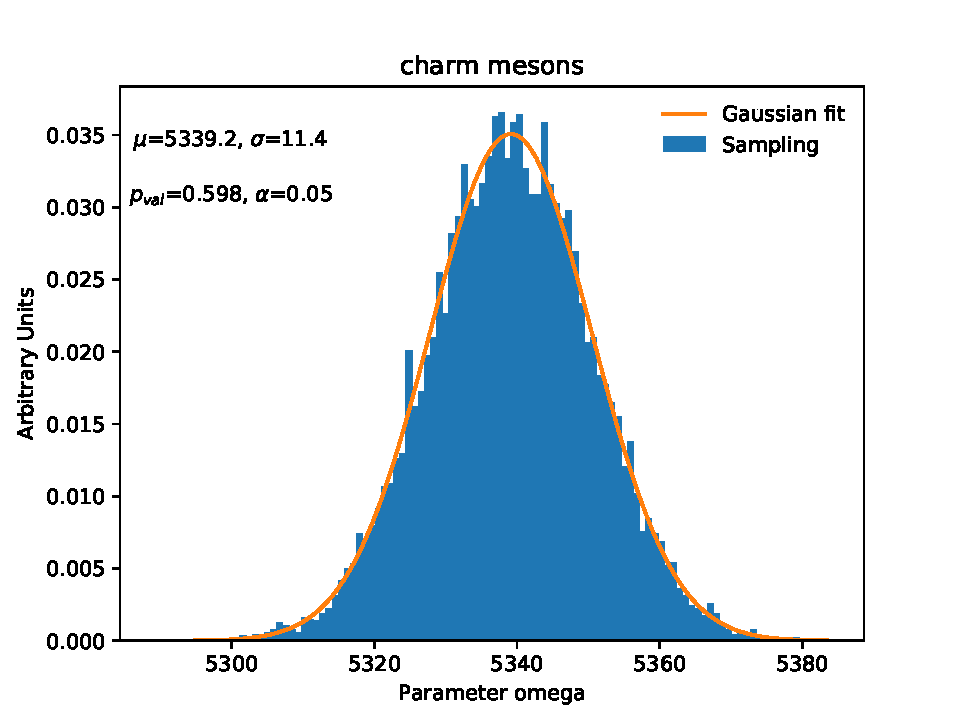
\includegraphics[scale=0.325]{./Plots/charm_bootstrap_k_All.pdf}
   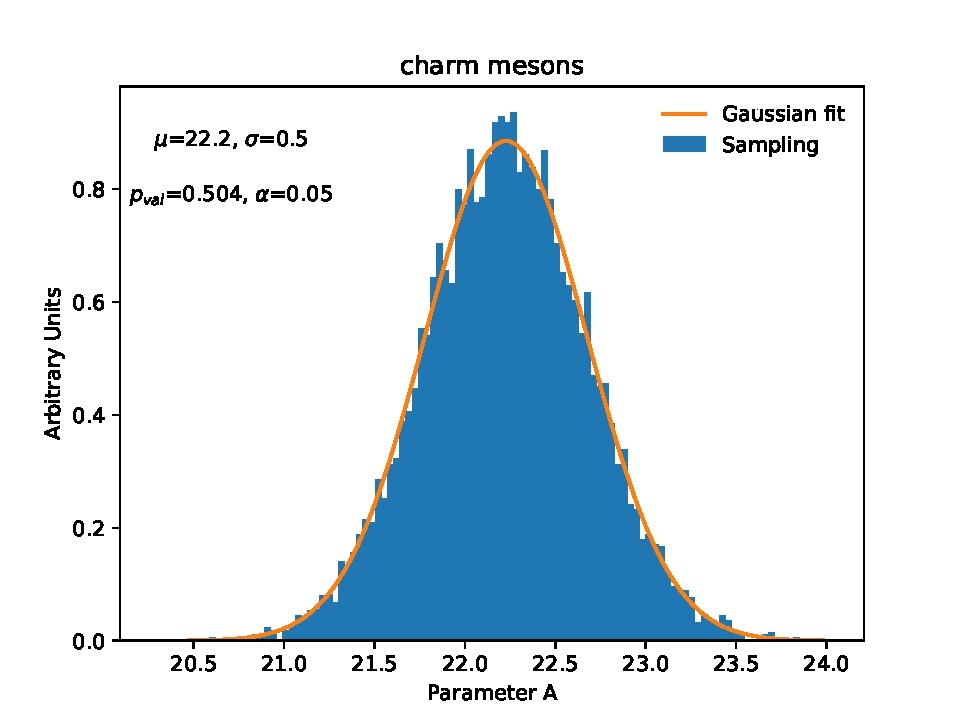
\includegraphics[scale=0.325]{./Plots/charm_bootstrap_a_All.pdf}       
\end{figure}

\end{frame}

\begin{frame}
\frametitle{Results: sampling distributions}
\scriptsize{A $p_{value}$ was obtained to formally test the null hypothesis of data being Gaussian distributed, with a $\alpha = 0.05$}
\begin{figure}
   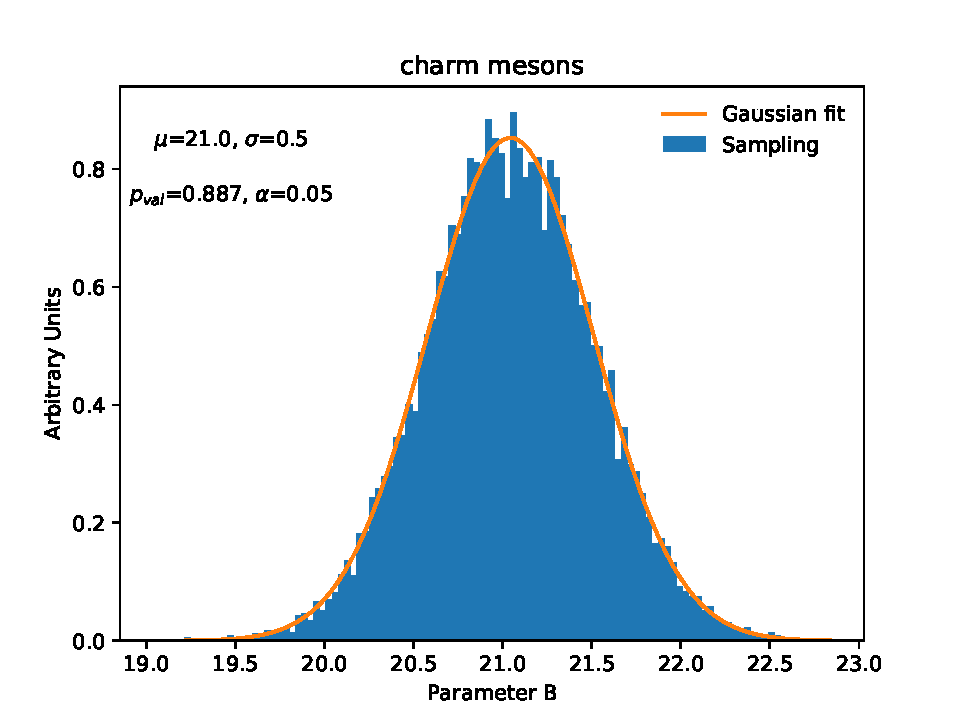
\includegraphics[scale=0.325]{./Plots/charm_bootstrap_b_All.pdf}
   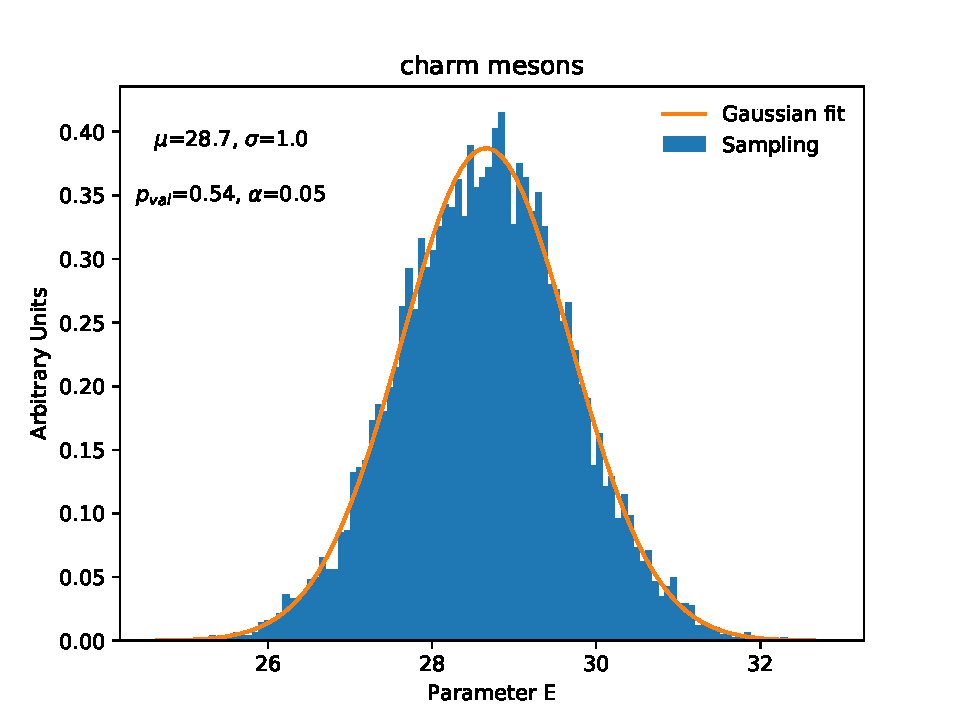
\includegraphics[scale=0.325]{./Plots/charm_bootstrap_e_All.pdf}   
\end{figure}

\end{frame}

\begin{frame}
\frametitle{Results: sampling distributions}
\scriptsize{A $p_{value}$ was obtained to formally test the null hypothesis of data being Gaussian distributed, with a $\alpha = 0.05$}
\begin{figure}
   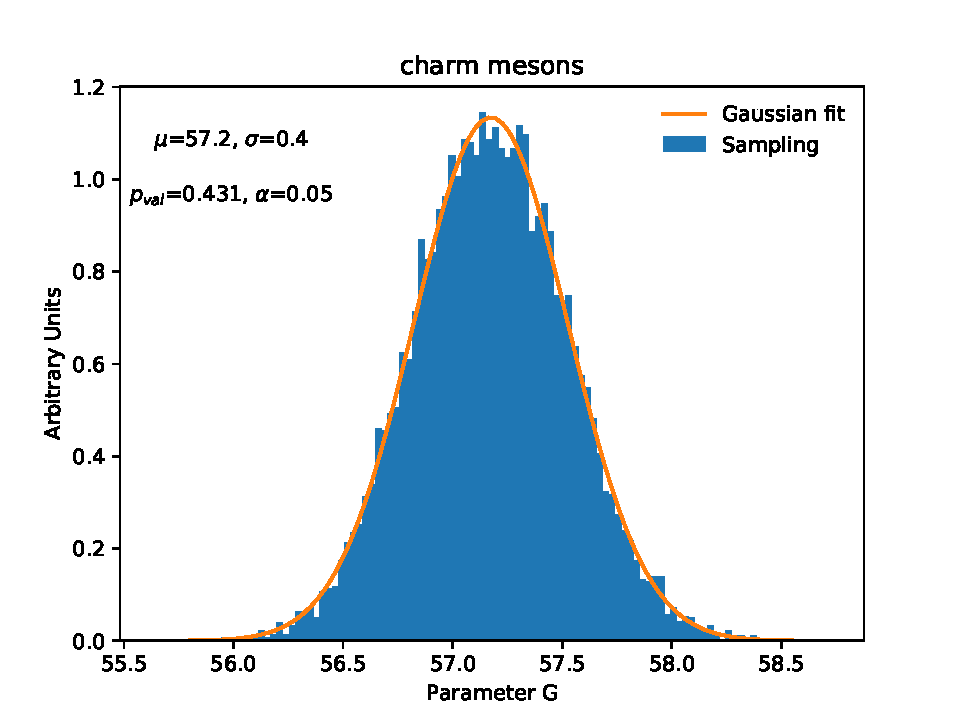
\includegraphics[scale=0.325]{./Plots/charm_bootstrap_g_All.pdf}
   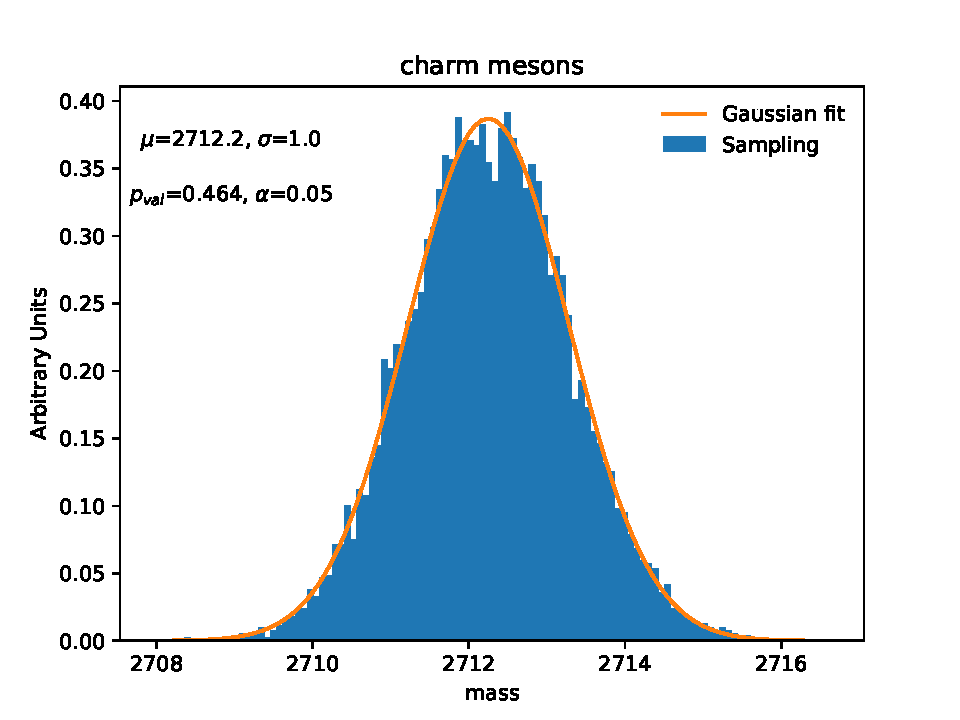
\includegraphics[scale=0.325]{./Plots/charm_bootstrap_mass_All.pdf}   
\end{figure}

\end{frame}



\section{Results}
\begin{frame}
\frametitle{Results: parameters}
\scriptsize{
\begin{table}[tb!]
\begin{center}
\begin{tabular}{c | c  c  c  c  c }\hline \hline
          & $K$        & $A$             & $B$     & $E$        & $G$            \\ \hline
Paper     & 5727.12$\pm x.xx$ & 21.54$\pm 0.37$ & 23.91$\pm 0.31$ & 30.34 $\pm 0.23$ & 54.37$\pm 0.58$ \\ 
Sampled   & 5339.2  $\pm 11.38 $ & 22.26  $\pm 0.46 $ & 21.07  $\pm 0.47 $ & 28.62  $\pm 1.02 $ & 57.16  $\pm 0.36 $ \\ 
L.Algebra & 5339.1  & 22.24  & 21.05  & 28.63 & 57.17  \\ 
\hline\hline
\end{tabular}
\caption{Model pararameters in MeV, for states: $ All $}

\begin{tabular}{c | c  c  c  c  c }\hline \hline
          & $K$        & $A$             & $B$     & $E$        & $G$            \\ \hline
Paper     & 5727.12$\pm x.xx$ & 21.54$\pm 0.37$ & 23.91$\pm 0.31$ & 30.34 $\pm 0.23$ & 54.37$\pm 0.58$ \\ 
Sampled   & 5995.1  $\pm 26.74 $ & 26.79  $\pm 0.48 $ & 31.92  $\pm 0.52 $ & 0.0  $\pm 0.0 $ & 49.56  $\pm 0.54 $ \\ 
L.Algebra & 5994.5  & 26.8  & 31.93  & 0.0 & 49.56  \\ 
\hline\hline
\end{tabular}
\caption{Model pararameters in MeV, for states: $ omega $}

\end{center}
\end{table}
}
\end{frame}

\section{Results}
\begin{frame}
\frametitle{Results: parameters}
\scriptsize{
\begin{table}[tb!]
\begin{center}
\begin{tabular}{c | c  c  c  c  c }\hline \hline
          & $K$        & $A$             & $B$     & $E$        & $G$            \\ \hline
Paper     & 5727.12$\pm x.xx$ & 21.54$\pm 0.37$ & 23.91$\pm 0.31$ & 30.34 $\pm 0.23$ & 54.37$\pm 0.58$ \\ 
Sampled   & 5463.8  $\pm 30.43 $ & 20.99  $\pm 0.7 $ & 23.82  $\pm 0.73 $ & 34.87  $\pm 4.75 $ & 56.76  $\pm 1.11 $ \\ 
L.Algebra & 5462.3  & 21.0  & 23.82  & 35.04 & 56.73  \\ 
\hline\hline
\end{tabular}
\caption{Model pararameters in MeV, for states: $ cascades $}

\begin{tabular}{c | c  c  c  c  c }\hline \hline
          & $K$        & $A$             & $B$     & $E$        & $G$            \\ \hline
Paper     & 5727.12$\pm x.xx$ & 21.54$\pm 0.37$ & 23.91$\pm 0.31$ & 30.34 $\pm 0.23$ & 54.37$\pm 0.58$ \\ 
Sampled   & 5013.3  $\pm 30.7 $ & 17.93  $\pm 0.92 $ & 14.93  $\pm 1.06 $ & 43.19  $\pm 2.5 $ & 50.81  $\pm 0.99 $ \\ 
L.Algebra & 5013.6  & 17.93  & 14.92  & 43.23 & 50.8  \\ 
\hline\hline
\end{tabular}
\caption{Model pararameters in MeV, for states: $ sigma_lamb $}

\end{center}
\end{table}
}
\end{frame}



\begin{frame}
\frametitle{\small{Masses, asymmetric errors calculated via 68\% quantile method}}
\vspace{-3mm}
\tiny{
\begin{table}[tb!]
\begin{tabular}{c | c  c  c  c  c}\hline \hline
Mass State & Experiment  &   Predicted mass  &    Predicted mass & diff pred & diff sampl\\ 
           & (MeV)       &   old (MeV)       &    sampled (MeV)  &     (\%) &     (\%)  \\ \hline
$\vert ssc,1/2,1/2,0,0,10/3 \rangle$ & 2695.0 $\pm 2.0 $  & 2702.4 $\pm xx$  & \textcolor{red}{ 2712.2  $^{+ 1.0 }_{ -1.0 }$}  &   -7.4 ( 0.3 )  &   -17.2 ( 0.6 ) \\  
$\vert ssc,3/2,3/2,0,0,10/3 \rangle$ & 2766.0 $\pm 2.0 $  & 2767.0 $\pm xx$  & \textcolor{red}{ 2779.0  $^{+ 1.4 }_{ -1.4 }$}  &   -1.0 ( 0.0 )  &   -13.0 ( 0.5 ) \\  
$\vert ssc,1/2,1/2,1,0,10/3 \rangle$ & 3000.4 $\pm 0.4 $  & 3015.8 $\pm xx$  & \textcolor{blue}{ 3005.6  $^{+ 1.0 }_{ -1.0 }$}  &   -15.4 ( 0.5 )  &   -5.2 ( 0.2 ) \\  
$\vert ssc,1/2,3/2,1,0,10/3 \rangle$ & 3050.2 $\pm 0.3 $  & 3044.5 $\pm xx$  & \textcolor{red}{ 3040.8  $^{+ 0.4 }_{ -0.4 }$}  &   5.7 ( 0.2 )  &   9.4 ( 0.3 ) \\  
$\vert ssc,3/2,1/2,1,0,10/3 \rangle$ & 3065.6 $\pm 0.4 $  & 3051.6 $\pm xx$  & \textcolor{red}{ 3037.2  $^{+ 0.6 }_{ -0.5 }$}  &   14.0 ( 0.5 )  &   28.4 ( 0.9 ) \\  
$\vert ssc,1/2,1/2,0,0,10/3 \rangle$ & 3090.2 $\pm 0.7 $  & 3080.4 $\pm xx$  & \textcolor{red}{ 3072.4  $^{+ 0.6 }_{ -0.6 }$}  &   9.8 ( 0.3 )  &   17.8 ( 0.6 ) \\  
$\vert suc,1/2,1/2,0,1/2,10/3 \rangle$ & 2578.0 $\pm 2.9 $  & 2570.1 $\pm xx$  & \textcolor{blue}{ 2578.7  $^{+ 1.0 }_{ -1.1 }$}  &   7.9 ( 0.3 )  &   -0.7 ( 0.0 ) \\  
$\vert suc,3/2,3/2,0,1/2,10/3 \rangle$ & 2645.9 $\pm 0.6 $  & 2634.8 $\pm xx$  & \textcolor{blue}{ 2645.5  $^{+ 0.9 }_{ -0.9 }$}  &   11.1 ( 0.4 )  &   0.4 ( 0.0 ) \\  
$\vert suc,1/2,3/2,1,1/2,10/3 \rangle$ & 2923.0 $\pm 0.4 $  & 2934.1 $\pm xx$  & \textcolor{blue}{ 2927.5  $^{+ 1.0 }_{ -1.0 }$}  &   -11.1 ( 0.4 )  &   -4.5 ( 0.2 ) \\  
$\vert suc,3/2,1/2,1,1/2,10/3 \rangle$ & 2938.5 $\pm 0.3 $  & 2941.2 $\pm xx$  & \textcolor{red}{ 2924.0  $^{+ 0.7 }_{ -0.8 }$}  &   -2.7 ( 0.1 )  &   14.5 ( 0.5 ) \\  
$\vert suc,3/2,3/2,1,1/2,10/3 \rangle$ & 2964.9 $\pm 0.3 $  & 2969.9 $\pm xx$  & \textcolor{red}{ 2959.1  $^{+ 0.6 }_{ -0.6 }$}  &   -5.0 ( 0.2 )  &   5.8 ( 0.2 ) \\  
$\vert uuc,1/2,1/2,0,1,10/3 \rangle$ & 2453.9 $\pm 0.1 $  & 2453.1 $\pm xx$  & \textcolor{red}{ 2459.5  $^{+ 1.9 }_{ -2.0 }$}  &   0.8 ( 0.0 )  &   -5.6 ( 0.2 ) \\  
$\vert uuc,3/2,3/2,0,1,10/3 \rangle$ & 2518.0 $\pm 2.3 $  & 2517.7 $\pm xx$  & \textcolor{red}{ 2526.3  $^{+ 1.3 }_{ -1.4 }$}  &   0.3 ( 0.0 )  &   -8.3 ( 0.3 ) \\  
$\vert uuc,1/2,1/2,1,1,10/3 \rangle$ & 2801.0 $\pm 6.0 $  & 2819.0 $\pm xx$  & \textcolor{blue}{ 2802.0  $^{+ 2.5 }_{ -2.6 }$}  &   -18.0 ( 0.6 )  &   -1.0 ( 0.0 ) \\  
$\vert udc,1/2,1/2,0,0,4/3  \rangle$ & 2286.5 $\pm 0.1 $  & 2283.7 $\pm xx$  & \textcolor{blue}{ 2287.9  $^{+ 0.4 }_{ -0.4 }$}  &   2.8 ( 0.1 )  &   -1.4 ( 0.1 ) \\  
$\vert udc,1/2,1/2,1,0,10/3 \rangle$ & 2592.3 $\pm 0.4 $  & 2649.7 $\pm xx$  & \textcolor{blue}{ 2630.4  $^{+ 0.8 }_{ -0.7 }$}  &   -57.4 ( 2.2 )  &   -38.1 ( 1.5 ) \\  
$\vert udc,3/2,1/2,1,0,4/3  \rangle$ & 2625.0 $\pm 0.2 $  & 2685.6 $\pm xx$  & \textcolor{blue}{ 2662.0  $^{+ 0.4 }_{ -0.4 }$}  &   -60.6 ( 2.3 )  &   -37.0 ( 1.4 ) \\  
$\vert ssc,1/2,1/2,0,1/2,4/3 \rangle$ & 2469.0 $\pm 4.0 $  & 2461.2 $\pm xx$  & \textcolor{blue}{ 2464.4  $^{+ 0.6 }_{ -0.6 }$}  &   7.8 ( 0.3 )  &   4.6 ( 0.2 ) \\  
$\vert ssc,1/2,1/2,1,1/2,4/3 \rangle$ & 2792.0 $\pm 3.3 $  & 2796.5 $\pm xx$  & \textcolor{red}{ 2778.0  $^{+ 1.3 }_{ -1.3 }$}  &   -4.5 ( 0.2 )  &   14.0 ( 0.5 ) \\  
$\vert ssc,3/2,1/2,1,1/2,10/3 \rangle$ & 2815.0 $\pm 0.2 $  & 2832.4 $\pm xx$  & \textcolor{blue}{ 2809.7  $^{+ 0.8 }_{ -0.8 }$}  &   -17.4 ( 0.6 )  &   5.3 ( 0.2 ) \\  
\hline
  &  &  & Total diff &  261.0  & 232.2 \\ 
\hline \hline
\end{tabular}
\caption{Every quantity is in MeV, except for percentage differences. States: All }

\end{table}
}
\end{frame}


\begin{frame}
\frametitle{\small{Masses, asymmetric errors calculated via 68\% quantile method}}
\tiny{
\begin{table}[tb!]
\begin{tabular}{c | c  c  c  c  c}\hline \hline
Mass State & Experiment  &   Predicted mass  &    Predicted mass & diff pred & diff sampl\\ 
           & (MeV)       &   old (MeV)       &    sampled (MeV)  &     (\%) &     (\%)  \\ \hline
$\vert ssc,1/2,1/2,0,0,10/3 \rangle$ & 2695.0 $\pm 2.0 $  & 2702.4 $\pm xx$  & \textcolor{blue}{ 2690.3  $^{+ 1.6 }_{ -1.6 }$}  &   -7.4 ( 0.3 )  &   4.7 ( 0.2 ) \\  
$\vert ssc,3/2,3/2,0,0,10/3 \rangle$ & 2766.0 $\pm 2.0 $  & 2767.0 $\pm xx$  & \textcolor{red}{ 2770.6  $^{+ 1.6 }_{ -1.6 }$}  &   -1.0 ( 0.0 )  &   -4.6 ( 0.2 ) \\  
$\vert ssc,1/2,1/2,1,0,10/3 \rangle$ & 3000.4 $\pm 0.4 $  & 3015.8 $\pm xx$  & \textcolor{blue}{ 3011.4  $^{+ 0.7 }_{ -0.8 }$}  &   -15.4 ( 0.5 )  &   -11.0 ( 0.4 ) \\  
$\vert ssc,1/2,3/2,1,0,10/3 \rangle$ & 3050.2 $\pm 0.3 $  & 3044.5 $\pm xx$  & \textcolor{red}{ 3043.9  $^{+ 0.3 }_{ -0.3 }$}  &   5.7 ( 0.2 )  &   6.3 ( 0.2 ) \\  
$\vert ssc,3/2,1/2,1,0,10/3 \rangle$ & 3065.6 $\pm 0.4 $  & 3051.6 $\pm xx$  & \textcolor{blue}{ 3059.3  $^{+ 0.4 }_{ -0.4 }$}  &   14.0 ( 0.5 )  &   6.3 ( 0.2 ) \\  
$\vert ssc,1/2,1/2,0,0,10/3 \rangle$ & 3090.2 $\pm 0.7 $  & 3080.4 $\pm xx$  & \textcolor{blue}{ 3091.8  $^{+ 0.8 }_{ -0.8 }$}  &   9.8 ( 0.3 )  &   -1.6 ( 0.1 ) \\  
\hline
  &  &  & Total diff &  53.0  & 34.6 \\ 
\hline \hline
\end{tabular}
\caption{Every quantity is in MeV, except for percentage differences. States: omega }

\end{table}
}
\end{frame}

\begin{frame}
\frametitle{\small{Masses, asymmetric errors calculated via 68\% quantile method}}
\tiny{
\begin{table}[tb!]
\begin{tabular}{c | c  c  c  c  c}\hline \hline
Mass State & Experiment  &   Predicted mass  &    Predicted mass & diff pred & diff sampl\\ 
           & (MeV)       &   old (MeV)       &    sampled (MeV)  &     (\%) &     (\%)  \\ \hline
$\vert suc,1/2,1/2,0,1/2,10/3 \rangle$ & 2578.0 $\pm 2.9 $  & 2570.1 $\pm xx$  & \textcolor{blue}{ 2581.1  $^{+ 2.2 }_{ -2.2 }$}  &   7.9 ( 0.3 )  &   -3.1 ( 0.1 ) \\  
$\vert suc,3/2,3/2,0,1/2,10/3 \rangle$ & 2645.9 $\pm 0.6 $  & 2634.8 $\pm xx$  & \textcolor{blue}{ 2644.0  $^{+ 1.3 }_{ -1.2 }$}  &   11.1 ( 0.4 )  &   1.9 ( 0.1 ) \\  
$\vert suc,1/2,3/2,1,1/2,10/3 \rangle$ & 2923.0 $\pm 0.4 $  & 2934.1 $\pm xx$  & \textcolor{blue}{ 2927.0  $^{+ 0.9 }_{ -0.9 }$}  &   -11.1 ( 0.4 )  &   -4.0 ( 0.1 ) \\  
$\vert suc,3/2,1/2,1,1/2,10/3 \rangle$ & 2938.5 $\pm 0.3 $  & 2941.2 $\pm xx$  & \textcolor{red}{ 2935.5  $^{+ 1.2 }_{ -1.2 }$}  &   -2.7 ( 0.1 )  &   3.0 ( 0.1 ) \\  
$\vert suc,3/2,3/2,1,1/2,10/3 \rangle$ & 2964.9 $\pm 0.3 $  & 2969.9 $\pm xx$  & \textcolor{blue}{ 2962.8  $^{+ 0.7 }_{ -0.7 }$}  &   -5.0 ( 0.2 )  &   2.1 ( 0.1 ) \\  
$\vert ssc,1/2,1/2,0,1/2,4/3 \rangle$ & 2469.0 $\pm 4.0 $  & 2461.2 $\pm xx$  & \textcolor{blue}{ 2467.6  $^{+ 2.3 }_{ -2.5 }$}  &   7.8 ( 0.3 )  &   1.4 ( 0.1 ) \\  
$\vert ssc,1/2,1/2,1,1/2,4/3 \rangle$ & 2792.0 $\pm 3.3 $  & 2796.5 $\pm xx$  & \textcolor{red}{ 2786.3  $^{+ 1.8 }_{ -1.8 }$}  &   -4.5 ( 0.2 )  &   5.7 ( 0.2 ) \\  
$\vert ssc,3/2,1/2,1,1/2,10/3 \rangle$ & 2815.0 $\pm 0.2 $  & 2832.4 $\pm xx$  & \textcolor{blue}{ 2822.0  $^{+ 1.1 }_{ -1.2 }$}  &   -17.4 ( 0.6 )  &   -7.0 ( 0.2 ) \\  
\hline
  &  &  & Total diff &  68.0  & 28.2 \\ 
\hline \hline
\end{tabular}
\caption{Every quantity is in MeV, except for percentage differences. States: cascades }

\end{table}
}
\end{frame}


\begin{frame}
\frametitle{\small{Masses, asymmetric errors calculated via 68\% quantile method}}
\tiny{
\begin{table}[tb!]
\begin{tabular}{c | c  c  c  c  c}\hline \hline
Mass State & Experiment  &   Predicted mass  &    Predicted mass & diff pred & diff sampl\\ 
           & (MeV)       &   old (MeV)       &    sampled (MeV)  &     (\%) &     (\%)  \\ \hline
$\vert uuc,1/2,1/2,0,1,10/3 \rangle$ & 2453.9 $\pm 0.1 $  & 2453.1 $\pm xx$  & \textcolor{red}{ 2464.2  $^{+ 1.6 }_{ -1.6 }$}  &   0.8 ( 0.0 )  &   -10.3 ( 0.4 ) \\  
$\vert uuc,3/2,3/2,0,1,10/3 \rangle$ & 2518.0 $\pm 2.3 $  & 2517.7 $\pm xx$  & \textcolor{blue}{ 2518.0  $^{+ 2.2 }_{ -2.3 }$}  &   0.3 ( 0.0 )  &   0.0 ( 0.0 ) \\  
$\vert uuc,1/2,1/2,1,1,10/3 \rangle$ & 2801.0 $\pm 6.0 $  & 2819.0 $\pm xx$  & \textcolor{blue}{ 2790.6  $^{+ 4.8 }_{ -4.8 }$}  &   -18.0 ( 0.6 )  &   10.4 ( 0.4 ) \\  
$\vert udc,1/2,1/2,0,0,4/3  \rangle$ & 2286.5 $\pm 0.1 $  & 2283.7 $\pm xx$  & \textcolor{red}{ 2276.2  $^{+ 1.6 }_{ -1.6 }$}  &   2.8 ( 0.1 )  &   10.3 ( 0.5 ) \\  
$\vert udc,1/2,1/2,1,0,10/3 \rangle$ & 2592.3 $\pm 0.4 $  & 2649.7 $\pm xx$  & \textcolor{blue}{ 2602.6  $^{+ 1.6 }_{ -1.6 }$}  &   -57.4 ( 2.2 )  &   -10.3 ( 0.4 ) \\  
$\vert udc,3/2,1/2,1,0,4/3  \rangle$ & 2625.0 $\pm 0.2 $  & 2685.6 $\pm xx$  & \textcolor{blue}{ 2625.0  $^{+ 0.2 }_{ -0.2 }$}  &   -60.6 ( 2.3 )  &   -0.0 ( 0.0 ) \\  
\hline
  &  &  & Total diff &  140.0  & 41.3 \\ 
\hline \hline
\end{tabular}
\caption{Every quantity is in MeV, except for percentage differences. States: sigma_lamb }

\end{table}
}
\end{frame}


\begin{frame}
\frametitle{Results: summary}

\begin{table}[tb!]
\begin{center}
\hspace{-6mm}
\hspace{-6mm}

\begin{tabular}{c  c  c  c  c  c}\hline \hline
     &  $K$      &     $A$   &      $B$   &      $E$  & $G$ \\ \hline
 $K$ &     1     &           &            &           &   \\ 
 $A$ & 0.24 &      1    &            &           &   \\ 
 $B$ & 0.43 & 0.46 &      1     &           &   \\ 
 $E$ & 0.1 & 0.1 & -0.03 &      1    &   \\ 
 $G$ & -0.53 & -0.71 & -0.23 & -0.49 & 1 \\ \hline \hline
\end{tabular}


\end{center}
\caption{Correlation matrix for the parameters}
\label{tab:summary}
\end{table}

\end{frame}







\section{Summary}

\begin{frame}
\frametitle{Summary and future work}
\begin{beamerboxesrounded}[upper=uppercolor, lower=lowercolor, shadow=true]{} 
\begin{itemize}

\item The bootstrap method was implemented successfully
\item Results look promising
\item Compute asymmetric uncertainties
\item More sampling statistical methods could be applied for comparison
\item Code is found on GitHub: \url{https://github.com/andrex-naranjas/flavor_phys}


\end{itemize}
\end{beamerboxesrounded}

\end{frame}





\begin{frame}

Thanks for listening!

\end{frame}


%\backupbegin
%\appendix 

\section{Backup}
\begin{frame}
\frametitle{Results: sampling distributions}

\begin{figure}
   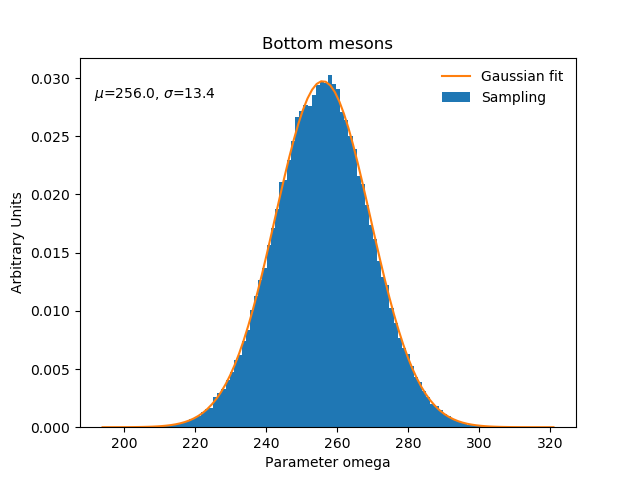
\includegraphics[scale=0.325]{./Plots/Bottom_bootstrap_o.png}
   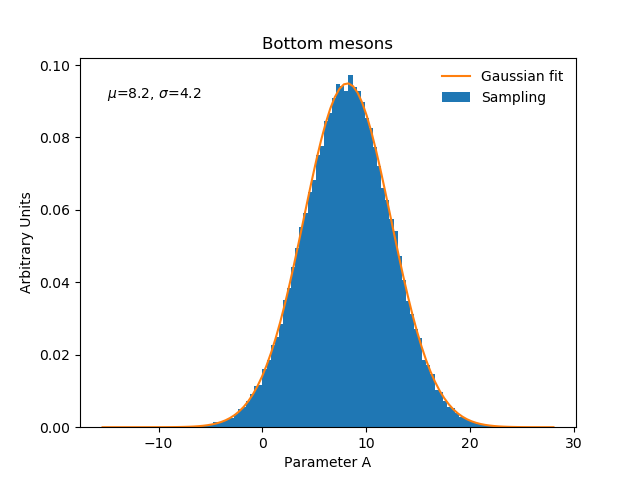
\includegraphics[scale=0.325]{./Plots/Bottom_bootstrap_a.png}       
\end{figure}

\end{frame}

\begin{frame}
\frametitle{Results: sampling distributions}
\begin{figure}
   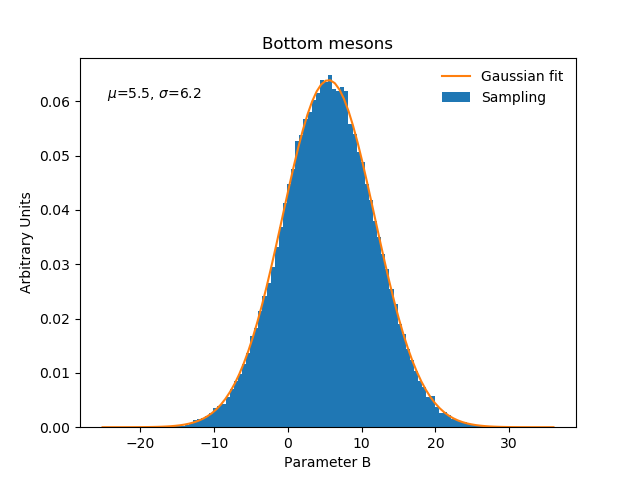
\includegraphics[scale=0.325]{./Plots/Bottom_bootstrap_b.png}
   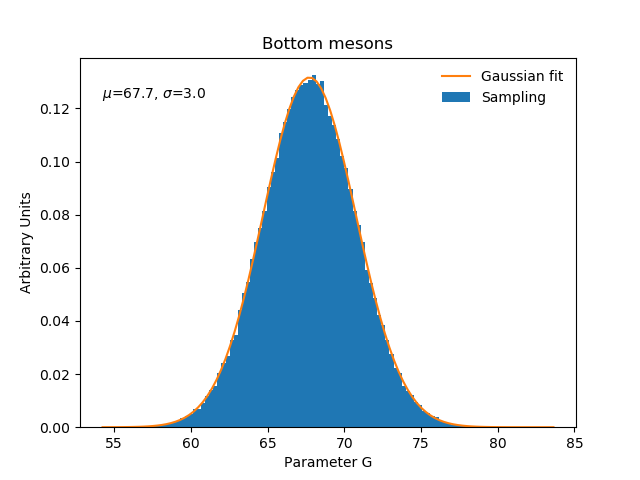
\includegraphics[scale=0.325]{./Plots/Bottom_bootstrap_g.png}       
\end{figure}

\end{frame}


\end{document}
